An extensive evaluation of Casanova implemented in Metacasanova, which we omit for brevity, can be found in \cite{DiGiacomo2017}. The implementation of Casanova operational semantics in Metacasanova is almost 5 times shorter than the corresponding F\# implementation in the hard-coded compiler. In addition to Casanova, we have implemented a subset of the C language called C-{}-. This language supports \texttt{if-then-else}, \texttt{while-loop}, and \texttt{for} statements, as well as local scoping of variables. The total length of the language definition in Metacasanova is 353 lines of code. The corresponding C\# code to implement the operational semantics of the language is 3123 lines, thus the code reduction with Metacasanova is roughly 8.84 times. For comparison, in Table \ref{tab:cmm} it is possible to see the code length to implement three different statements, both in Metacasanova and C\#. We tested C -{}- against Python by computing the average running time to compute the factorial of a number. C-{}- results to be 2 orders of magnitude slower than Python. This result is worse than what we obtained with Casanova, because in order to emulate the interruptible rule mechanism of Casanova in Python you must rely on coroutines that are slower than a program containing simple statements. Moreover, we tested the performance improvement of the optimization using Functors to represent records against the standard one using dynamic symbol tables. The test was run using records with a number of fields ranging from 1 to 10 and updating from 10000 to 1000000 instances of such records. The results can be seen in Table \ref{tab:functors} and Figure \ref{fig:chart}: the optimization using Functors leads to a performance increase on average of one order of magnitude over the implementation with dictionaries. In Figure \ref{fig:chart} we can also see that the performance of the dynamic table degrades considerably when increasing the number of fields, while the performance of the implementation with Functors is almost constant.  Note that the performance of the dynamic table is improved by the fact that we are using a dictionary implemented in .NET. If the symbol table is represented as a meta-data structure in the language the performance would be even worse, since it has to be encoded a list of pairs with the field name and its value.

\begin{table}	
	\caption{Running time with the functor optimization and the dynamic table.}
	\begin{tabular}{|c|c|c|c|}
		\hline
		\textbf{FIELDS}& \textbf{RECORDS}& \textbf{Functors (ms)}&\textbf{Dynamic Table (ms)}\\ \hline
		1&	10000&	1.00E-05& 5.00E-06\\ \hline
		1&	100000&	9.60E-05& 6.30E-05\\ \hline
		1&	1000000&	0.000947& 0.000729\\ \hline
		2&	10000&	9.00E-06& 1.30E-05\\ \hline
		2&	100000&	9.40E-05&0.000159\\ \hline
		2&	1000000&	0.000951&0.001783\\ \hline
		3&	10000&	9.00E-06&2.70E-05\\ \hline
		3&	100000&	9.50E-05&0.000304\\ \hline
		3&	1000000&	0.00095&0.003332\\ \hline
		4&	10000&	9.00E-06&4.50E-05\\ \hline
		4&	100000&	9.60E-05&0.000503\\ \hline
		4&	1000000&	0.00096&0.00543\\ \hline
		5&	10000&	9.00E-06&7.00E-05\\ \hline
		5&	100000&	9.60E-05&0.000752\\ \hline
		5&	1000000&	0.000965&0.008027\\ \hline
		6&	10000&	9.00E-06&9.90E-05\\ \hline
		6&	100000&	9.60E-05&0.001051\\ \hline
		6&	1000000&	0.000971&0.01111\\ \hline
		7&	10000&	9.00E-06&0.000133\\ \hline
		7&	100000&	9.70E-05&0.001413\\ \hline
		7&	1000000&	0.000975&0.014739\\ \hline
		8&	10000&	9.00E-06&0.000175\\ \hline
		8&	100000&	9.80E-05&0.001822\\ \hline
		8&	1000000&	0.000982&0.018931\\ \hline
		9&	10000&	9.00E-06&0.00022\\ \hline
		9&	100000&	9.90E-05&0.002294\\ \hline
		9&	1000000&	0.000992&0.023666\\ \hline
		10&	10000&	9.00E-06&0.00027\\ \hline
		10&	100000&	0.0001&	0.002805\\ \hline
		10&	1000000& 0.001004&	0.028732\\ \hline		
	\end{tabular}
	\label{tab:functors}
\end{table}

\begin{table}
	\centering
	\caption{Code length implementation of C-{}- and run-time performance}
	\begin{tabular}{|c|c|c|}
		\hline
		\textbf{Statement} & \textbf{Metacasanova} & \textbf{C\#}\\
		\hline
		\texttt{if-then-else} & 4 & 103 \\
		\hline
		\texttt{while} & 7 & 73 \\
		\hline
		\texttt{For} & 11 & 81\\
		\hline
	\end{tabular}
	\begin{tabular}{|c|c|}
		\hline
		\textbf{C-{}-} & \textbf{Python} \\
		\hline
		1.26ms & $2.36 \cdot 10^{-2}$ms \\
		\hline
	\end{tabular}
	\label{tab:cmm}
\end{table}

\begin{figure}
	\label{fig:chart}
	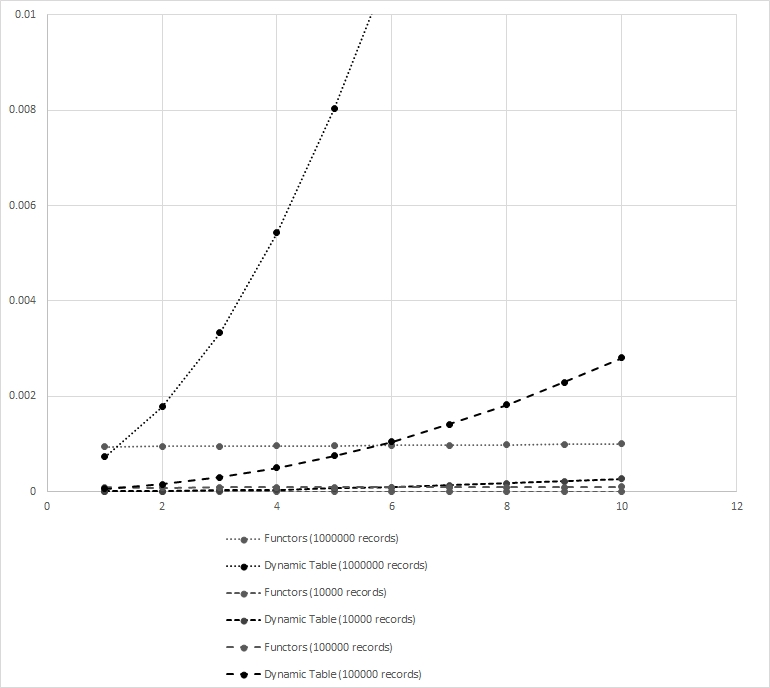
\includegraphics[width = \columnwidth]{Figures/chart.jpg}
	\caption{Execution time of the different memory models}
\end{figure}